\documentclass{article}\usepackage[]{graphicx}\usepackage[]{color}
%% maxwidth is the original width if it is less than linewidth
%% otherwise use linewidth (to make sure the graphics do not exceed the margin)
\makeatletter
\def\maxwidth{ %
  \ifdim\Gin@nat@width>\linewidth
    \linewidth
  \else
    \Gin@nat@width
  \fi
}
\makeatother

\definecolor{fgcolor}{rgb}{0.345, 0.345, 0.345}
\newcommand{\hlnum}[1]{\textcolor[rgb]{0.686,0.059,0.569}{#1}}%
\newcommand{\hlstr}[1]{\textcolor[rgb]{0.192,0.494,0.8}{#1}}%
\newcommand{\hlcom}[1]{\textcolor[rgb]{0.678,0.584,0.686}{\textit{#1}}}%
\newcommand{\hlopt}[1]{\textcolor[rgb]{0,0,0}{#1}}%
\newcommand{\hlstd}[1]{\textcolor[rgb]{0.345,0.345,0.345}{#1}}%
\newcommand{\hlkwa}[1]{\textcolor[rgb]{0.161,0.373,0.58}{\textbf{#1}}}%
\newcommand{\hlkwb}[1]{\textcolor[rgb]{0.69,0.353,0.396}{#1}}%
\newcommand{\hlkwc}[1]{\textcolor[rgb]{0.333,0.667,0.333}{#1}}%
\newcommand{\hlkwd}[1]{\textcolor[rgb]{0.737,0.353,0.396}{\textbf{#1}}}%

\usepackage{framed}
\makeatletter
\newenvironment{kframe}{%
 \def\at@end@of@kframe{}%
 \ifinner\ifhmode%
  \def\at@end@of@kframe{\end{minipage}}%
  \begin{minipage}{\columnwidth}%
 \fi\fi%
 \def\FrameCommand##1{\hskip\@totalleftmargin \hskip-\fboxsep
 \colorbox{shadecolor}{##1}\hskip-\fboxsep
     % There is no \\@totalrightmargin, so:
     \hskip-\linewidth \hskip-\@totalleftmargin \hskip\columnwidth}%
 \MakeFramed {\advance\hsize-\width
   \@totalleftmargin\z@ \linewidth\hsize
   \@setminipage}}%
 {\par\unskip\endMakeFramed%
 \at@end@of@kframe}
\makeatother

\definecolor{shadecolor}{rgb}{.97, .97, .97}
\definecolor{messagecolor}{rgb}{0, 0, 0}
\definecolor{warningcolor}{rgb}{1, 0, 1}
\definecolor{errorcolor}{rgb}{1, 0, 0}
\newenvironment{knitrout}{}{} % an empty environment to be redefined in TeX

\usepackage{alltt}

\usepackage[letterpaper, portrait, margin=1in]{geometry}
\usepackage{amsmath}
\usepackage{hyperref}

\title{MATH 680 - Assignment \#5}
\author{Kevin McGregor}
\date{December 21st, 2015}

\newcommand{\expit}{\frac{\exp(x_{it}^\top\beta+u_i)}{1+\exp(x_{it}^\top\beta+u_i)}}
\newcommand{\altexpit}{\frac{1}{1+\exp(x_{it}^\top\beta+u_i)}}
\newcommand{\lc}{\left(}
\newcommand{\rc}{\right)}
\newcommand{\lb}{\left\{}
\newcommand{\rb}{\right\}}
\newcommand{\smat}{\left(X^\top X +\lambda w I_p + \lambda(1-w)H\right)}
\newcommand{\mub}{\mu_B}
\IfFileExists{upquote.sty}{\usepackage{upquote}}{}
\begin{document}
\maketitle

\section*{Question 1}
\subsection*{(a)}
First we find the posterior distribution of the parameters:
\begin{equation*}
\begin{split}
  f(\beta,u,v_u | y) \propto \frac{1}{v_u^{n/2}} & \exp\lb\frac{-1}{2v_u}\sum_{i=1}^{n}u_i^2 \rb v_u^{-(\alpha_0-1)} e^{-\beta_0/v_u} \exp\lb\frac{-1}{2v_B}\sum_{i=1}^{p}\beta_j^2 \rb \\
  & \prod_{i=1}^n \prod_{t=1}^{T_i} \lc\expit\rc^{y_{it}} \lc\altexpit\rc^{1-y_{it}}.
\end{split}
\end{equation*}
The number of parameters we need to estimate is $p+n+1$, i.e., $p$ elements of $\beta$, $n$ elements of $u_i$, and $v_u$.  Our trial distribution on the $k^{th}$ iteration will be:
\begin{equation}
N_{p+n+1} \lc \begin{bmatrix} \beta_1 \\ \vdots \\ \beta_{p+n+1} \end{bmatrix} , 
  \begin{bmatrix} s_1^2 & 0 & \dots & 0 \\
                  0 & s_2^2 & & \vdots \\
                  \vdots & & \ddots & \\
                  0 & \dots & & s_{p+n+1}^2 \end{bmatrix} \rc
\label{eqn:norm}
\end{equation}
For convenience, we take the log of the posterior distribution:
\begin{equation*}
\begin{split}
  \log f(\beta,u,v_u | y) = -\frac{n}{2}\log(v_u) & \frac{-1}{2v_B}\sum_{i=1}^{p}\beta_j^2 -(\alpha_0-1)\log(v_u) - \frac{\beta_0}{v_u} - \frac{-1}{2v_B}\sum_{i=1}^{p}\beta_j^2 \\
  & + \sum_{i=1}^{n}\sum_{t=1}^{T_i} \lb y_{it}\log\lc\expit\rc + \lc 1-y_{it}\rc \log\lc\altexpit\rc \rb  .
\end{split}
\end{equation*}
If $v_u<0$ then set $\log f = -\infty$.  Next define:
\begin{equation*}
\begin{split}
  \log\alpha\lb(\beta_k,u_k,v_{uk}),(\beta_j,u_j,v_{uj})\rb = \min\lb 0, \log f (\beta_j,u_j,v_{uj}) - \log f (\beta_k,u_k,v_{uk})  \rb.
\end{split}
\end{equation*}
So, to begin the algorithm, we choose initial values $\beta_0$, $u_0$, and $v_{u0}$, and set $k=0$.  The algorithm proceeds as follows:
\begin{enumerate}
  \item Generate $Z$ as specified in \ref{eqn:norm}, and $U\sim U(0,1)$.
  \item If $\log U < \log\alpha\lb(\beta_k,u_k,v_{uk}),Z)\rb$, set $(\beta_{k+1},u_{k+1},v_{u(k+1)}) = Z$. Otherwise set $(\beta_{k+1},u_{k+1},v_{u(k+1)}) = (\beta_k,u_k,v_{uk})$.
  \item Set $k=k+1$ and go to step (1).
\end{enumerate}

\subsection*{(b)}
\emph{The code for the R function for part (a) can be found in bern\_mcmc.R}

\subsection*{(c)}
\begin{knitrout}
\definecolor{shadecolor}{rgb}{0.969, 0.969, 0.969}\color{fgcolor}\begin{figure}
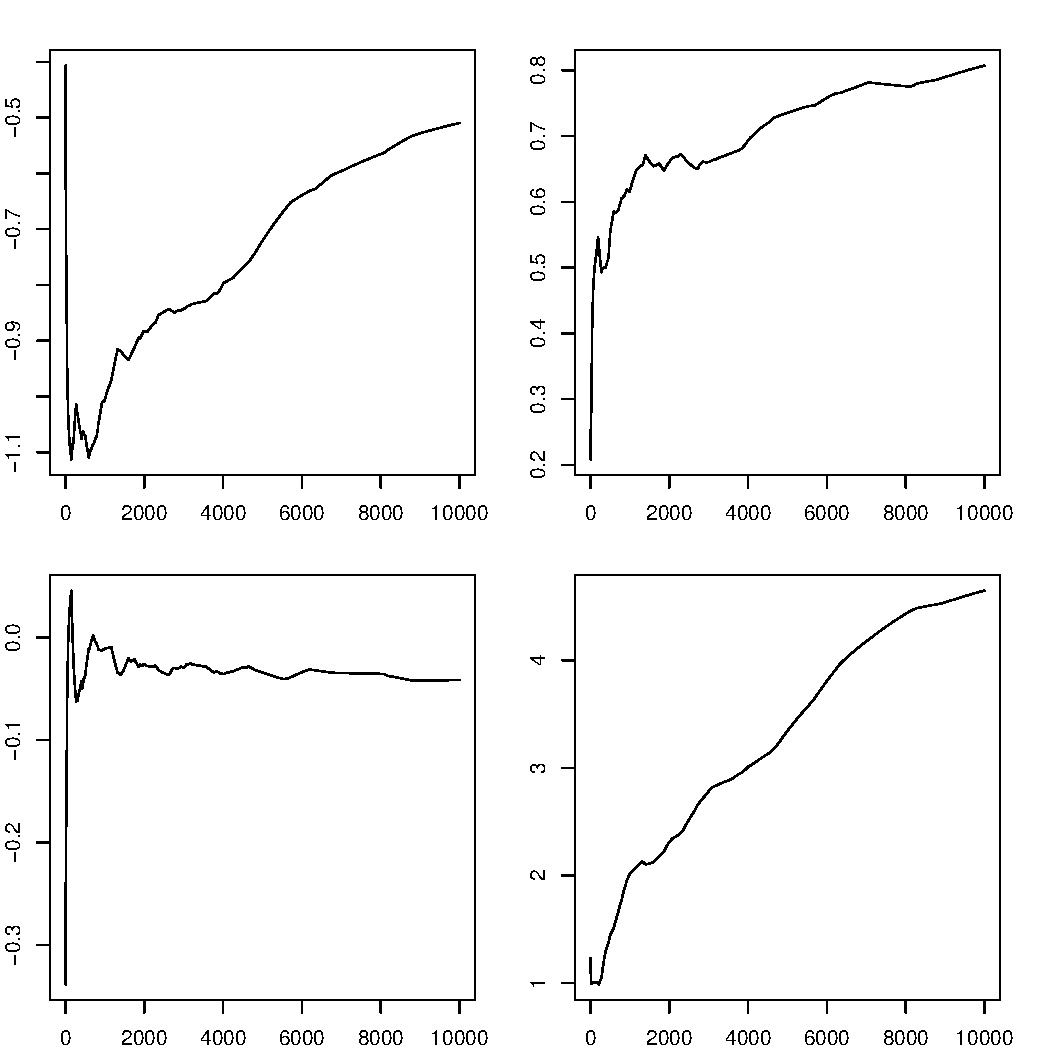
\includegraphics[width=\maxwidth]{figure/trace1-1} \caption[Trace plots for the elements of beta and ]{Trace plots for the elements of beta and $v_u$ (Part (c))}\label{fig:trace1}
\end{figure}


\end{knitrout}

\emph{Code for this part can be found in the file a5\_q1.R}. The trace plots for this function can be found in Figure~\ref{fig:trace1}.  As we can see, the trace plots do not look like convergence has been achieved yet; estimates could be improved.  This is unsurprising due to the inefficienty of the algorithm.  This algorithm would need to perform many more samples before proper convergence would be achieved.  Estimated standard errors for $E(B|Y=y)$ are $(0.29, 0.15, 0.07)$.

\subsection*{(d)}
\begin{knitrout}
\definecolor{shadecolor}{rgb}{0.969, 0.969, 0.969}\color{fgcolor}\begin{figure}
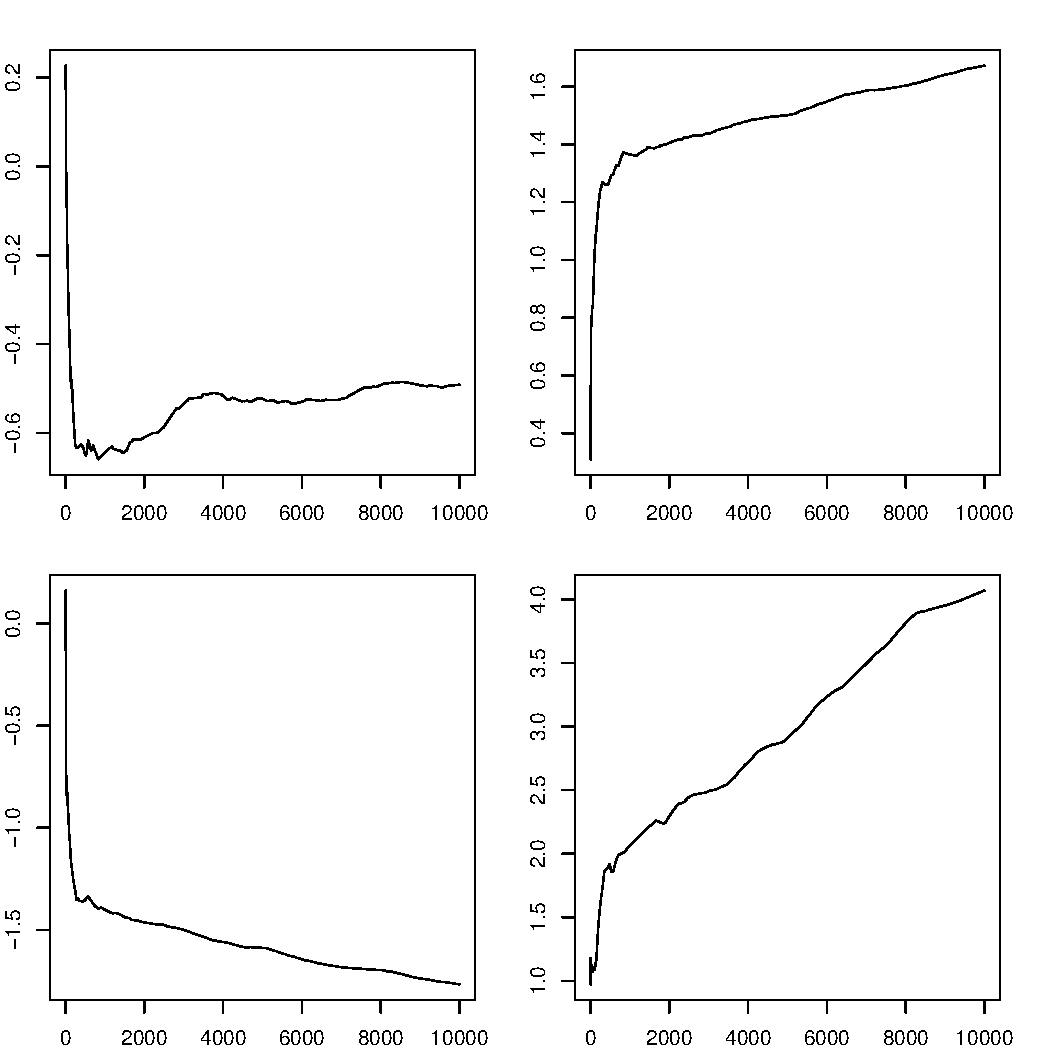
\includegraphics[width=\maxwidth]{figure/trace2-1} \caption[Trace plots for the elements of beta and ]{Trace plots for the elements of beta and $v_u$ (Part (d))}\label{fig:trace2}
\end{figure}


\end{knitrout}

\emph{Code for this part can be found in the file a5\_q1.R} The values I chose for this problem are: $n=100$, $p=2$, $T_i=15$ for all $i$, $\beta=(1,2,-2)^\top$, $v_u=1$.  Trace plots for this example can be found in Figure~\ref{fig:trace2}, and as before, convergence has not been reached and estimates could be improved.

\section*{Question 2}
\subsection*{(a)}
\emph{Code for this part can be found in the file fusedRidge\_crossval.R}.

\subsection*{(b)}
\begin{equation*}
\begin{split}
  f(\beta,v,\lambda | y) \propto \frac{1}{v^{n/2}} & \exp\lb-\frac{1}{2v}(y-X\beta)^\top(y-X\beta)\rb  \frac{\lambda^{p/2}}{v^{p/2}} \exp\lb-\beta^\top\frac{\lambda}{2v}(wI_p+(1-w)H)\beta\rb \\
  & v^{-a_v-1}e^{-b_v/v}\lambda^{a_L-1}e^{-b_L\lambda}.
\end{split}
\end{equation*}
Now, 
\begin{eqnarray*}
  f(\beta | v,\lambda,y) &\propto& \exp\lb -\frac{1}{2v}(y^\top y - 2\beta^\top X^\top y + \beta^\top X^\top X \beta + \beta^\top\lambda w I_p\beta + \beta^\top\lambda(1-w)H\beta) \rb \\
  &\propto & \exp\lb -\frac{1}{2v}\beta^\top\smat\beta + \frac{1}{v}\beta^\top(X^\top y) \rb.
\end{eqnarray*}
Therefore,
\begin{eqnarray*}
  (B | V=v,L=\lambda,Y=y) & \sim & N_p\left( \smat^{-1}(X^\top y), v\smat^{-1} \right).
\end{eqnarray*}
Then, if we let $\mub = \smat^{-1}(X^\top y)$, we have:
\begin{eqnarray*}
  f(\beta | v,\lambda,y) &\propto_{\beta,v}& \exp\lb -\frac{1}{2v}\left( \beta^\top\smat\beta -2\beta^\top(X^\top y) + \mub^\top\smat\mub \right) \rb,
\end{eqnarray*}
and so,
\begin{eqnarray*}
  f(\beta, v | \lambda,y) &\propto_{\beta,v}& v^{-(n/2+p/2+a_v+1)}\exp\lb \frac{1}{2v}\left( y^\top y - 2\beta^\top X^\top y + \beta^\top X^\top X \beta + \lambda\beta^\top(wI_p+(1-w)H)\beta+2b_v \right) \rb \\
  &=& f(\beta|v,\lambda,y) v^{-(n/2+a_v+1)}\exp\lb-\frac{1}{2v}\left[y^\top y - \mub^\top\smat\mub+2b_v\right] \rb.
\end{eqnarray*}
Therefore,
\begin{eqnarray*}
  (V | L=\lambda,Y=y) &\sim& \mbox{InvGam}\left(a_v+\frac{n}{2}, b_v + \frac{1}{2}\left[y^\top y - \mub^\top\smat\mub+2b_v\right] \right).
\end{eqnarray*}
Finally,
\begin{eqnarray*}
  f(\lambda | \beta,v,y) &\propto& \lambda^{p/2+a_L-1}\exp\lb-\lambda\left( \frac{1}{2v}\beta^\top (wI_p+(1-w)H) \beta +b_L \right)\rb, 
\end{eqnarray*}
and so,
\begin{eqnarray*}
  (L | B=\beta,V=v,Y=y) &\sim& \mbox{Gamma}\left(\frac{p}{2}+a_l, \frac{1}{2v}\beta^\top(wI_p+(1-w)H)\beta + b_L\right). 
\end{eqnarray*}
The algorithm begins by picking $(\beta_0, v_0, \lambda_0)$, and setting $k=0$.  The algorithm procees as follows:
\begin{enumerate}
  \item Generate $v_{k+1}$ from $(V | L=\lambda_k,Y=y)$ and $\beta_{k+1}$ from $(B | V=v_{k+1},L=\lambda_{k+1},Y=y)$.
  \item Generate $\lambda_{k+1}$ from $(L | B=\beta_{k+1},V=v_{k+1},Y=y)$.
  \item Set $k=k+1$, and go to step (1).
\end{enumerate}

Running the algorithm in R (\emph{see file a5\_q2bii.R}), we see estimates for beta and credible intervals in Table~\ref{tab:q2est}

\begin{table}[ht]
\centering
\begin{tabular}{cccc}
  \hline
  Truth & Estimate & Lower & Upper \\ 
  \hline
1.0000 & 0.8274 & 0.1305 & 1.5504 \\ 
  1.0000 & 0.9986 & 0.1586 & 1.8350 \\ 
  0.7500 & 0.9400 & 0.0409 & 1.8285 \\ 
  0.5000 & -0.0318 & -1.0351 & 0.9343 \\ 
  0.5000 & 0.9247 & 0.2412 & 1.5966 \\ 
   \hline
\end{tabular}
\caption{Estimated values and credible intervals for $\beta$}
\label{tab:q2est}
\end{table}

We can also see the trace plots in Figure~\ref{fig:trace3}.  Convergence appears to have been reached for all elements.  Figure~\ref{fig:acf1} shows the autocorrelation of the mean of the elements of beta over the different iterations.  The autocorrelation is very small, even for smaller lags.

\begin{knitrout}
\definecolor{shadecolor}{rgb}{0.969, 0.969, 0.969}\color{fgcolor}\begin{figure}
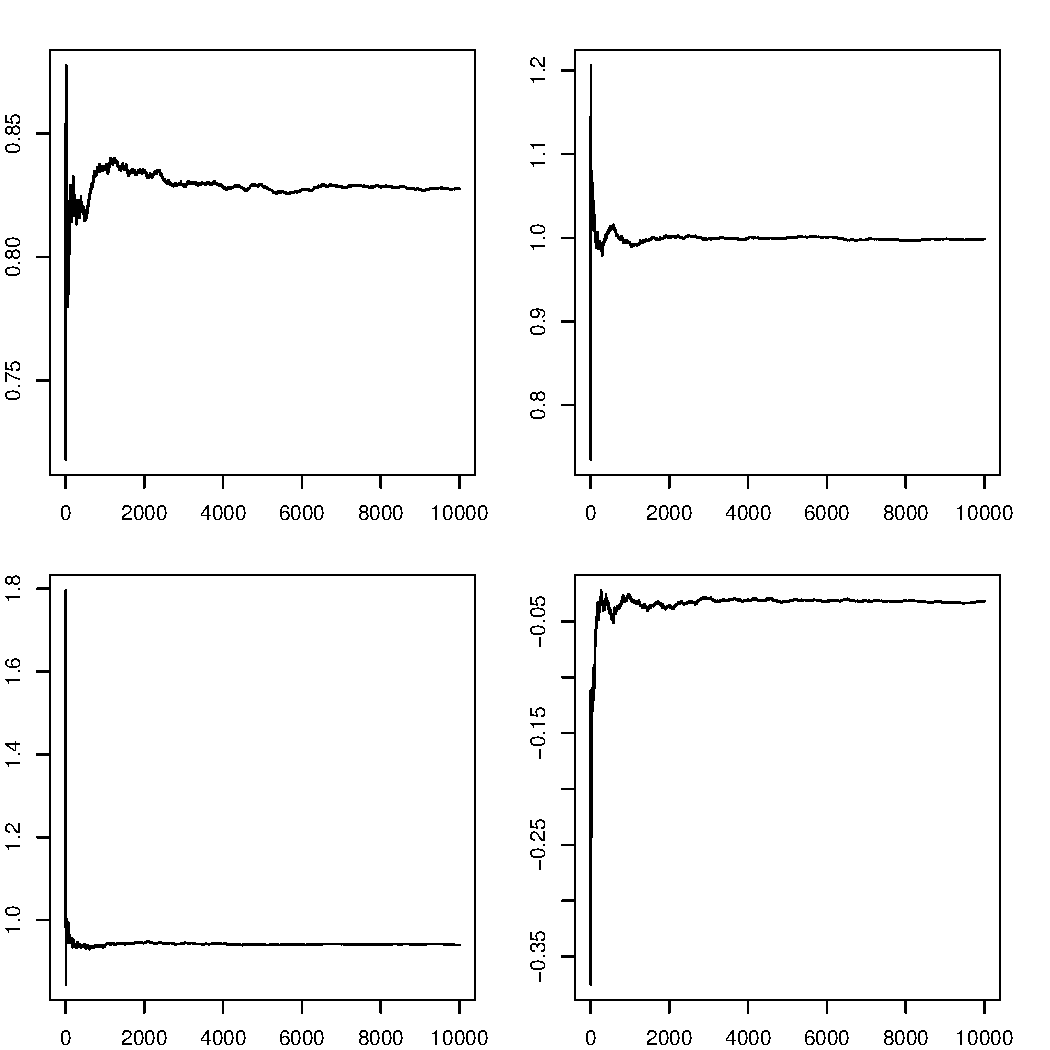
\includegraphics[width=\maxwidth]{figure/trace3-1} \caption[Trace plots for the first 4 elements of beta]{Trace plots for the first 4 elements of beta}\label{fig:trace3}
\end{figure}


\end{knitrout}

\begin{knitrout}
\definecolor{shadecolor}{rgb}{0.969, 0.969, 0.969}\color{fgcolor}\begin{figure}
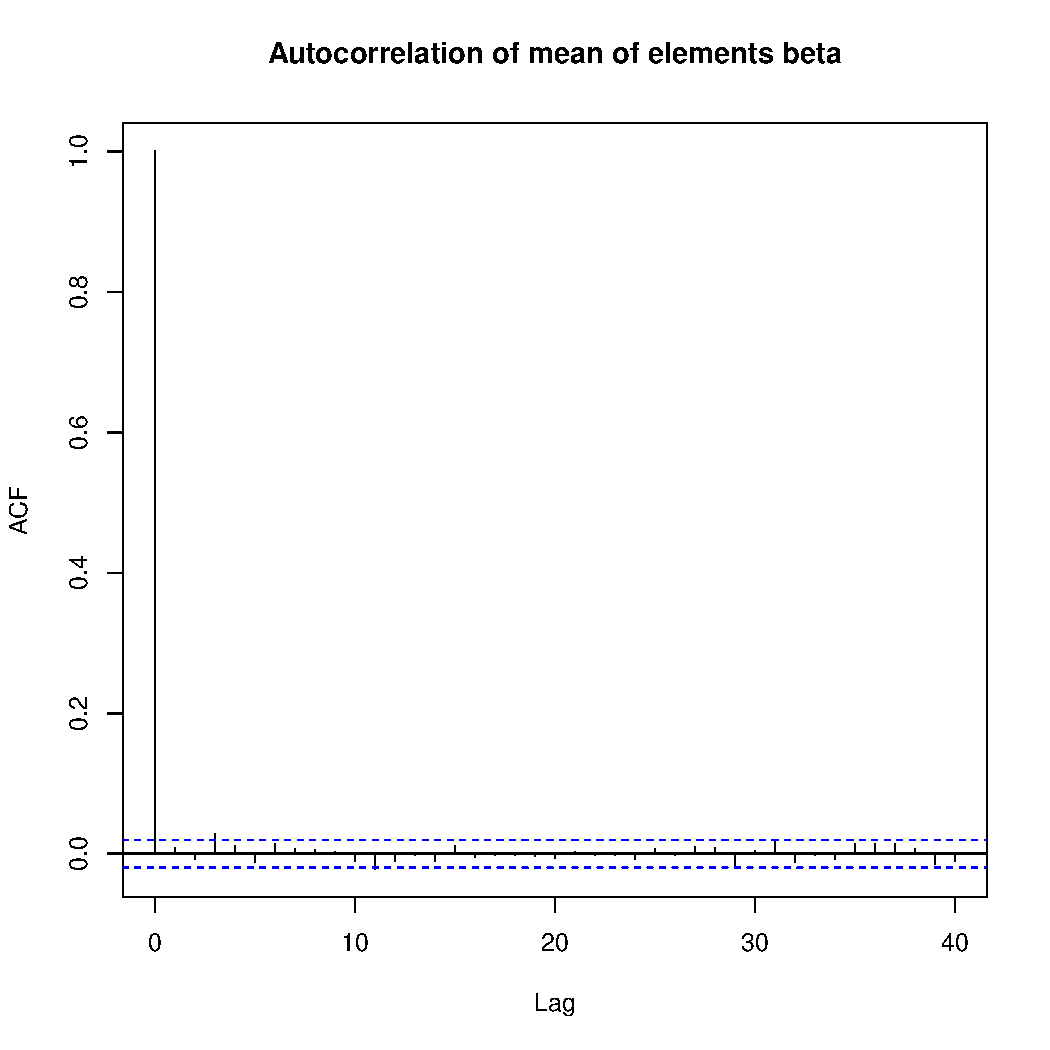
\includegraphics[width=\maxwidth]{figure/acf1-1} \caption[Plotting the autocorrelation for the mean of the estimated elements of beta]{Plotting the autocorrelation for the mean of the estimated elements of beta}\label{fig:acf1}
\end{figure}


\end{knitrout}

\section*{Question 3}
\subsection*{(a)}
We use Metropolis-Hastings sampling to sample from $\mbox{Beta}(\alpha,\beta)$ with a uniform trial density.

If $X\sim \mbox{Beta}(\alpha,\beta)$, then:
\begin{eqnarray*}
  f_X(x) &=& \frac{1}{B(\alpha,\beta)}x^{\alpha-1}(1-x)^{\beta-1}, \mbox{ for } x\in(0,1).
\end{eqnarray*}
Then, for some $b\in (0,1)$, sample from the following trial distribution at every sample $x_k$: $$ Z\sim U(x_k-b,x_k+b) $$
Now, let 
\begin{eqnarray*}
  \alpha(x,y) &=& \min\lb 1, \left(\frac{y}{x}\right)^{\alpha-1}\left(\frac{1-y}{1-x}\right)^{\beta-1} \rb, \mbox{ for } y\in (0,1).
\end{eqnarray*}
So, simply generate $U\sim U(0,1)$, and accept the new sample (set $x_{k+1}=Z$) if $U<\alpha(x_k, Z)$.

\subsection*{(b)}
\emph{Testing for this function (as well as the function itself) can be found in the file sampleBeta.R}.  Trace plots for two runs of this function (on different parameter values), can be seen in Figure~\ref{fig:trace_q3}.  Convergence to the theoretical mean has been achieved in both cases.

\begin{knitrout}
\definecolor{shadecolor}{rgb}{0.969, 0.969, 0.969}\color{fgcolor}\begin{figure}
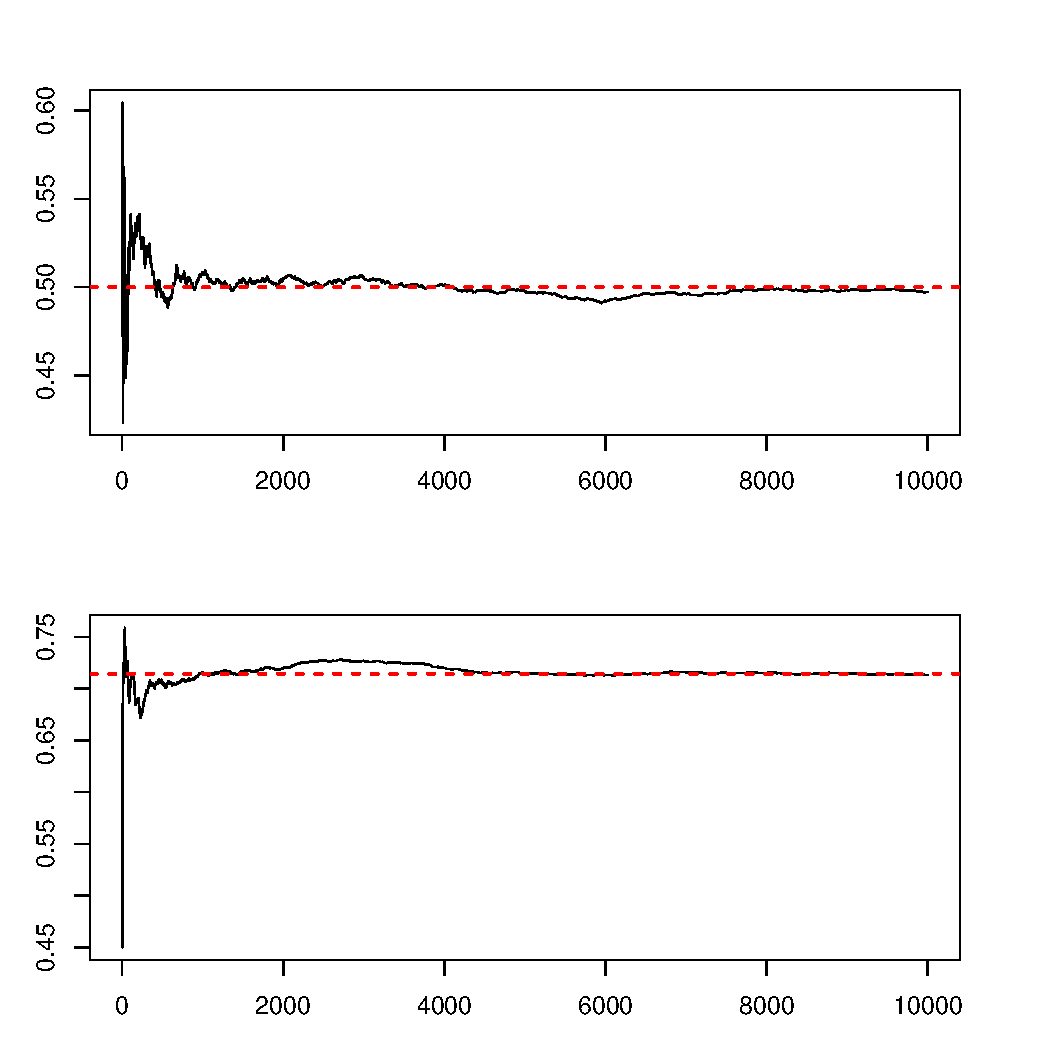
\includegraphics[width=\maxwidth]{figure/trace_q3-1} \caption[Trace plots for the means of two samples for the beta distribution (two different sets of parameters)]{Trace plots for the means of two samples for the beta distribution (two different sets of parameters).  The red line represents the theoretical mean}\label{fig:trace_q3}
\end{figure}


\end{knitrout}

We can also look at the autocorrelation plots for these two parameter scenarios.  This can be seen in Figure~\ref{fig:acf_q3}.  The autocorrelation declines rapidly, but seems to alternate between very small positive and negative correlations.  Perhaps this has something to do with the boundedness of the beta distribution's support.

\begin{knitrout}
\definecolor{shadecolor}{rgb}{0.969, 0.969, 0.969}\color{fgcolor}\begin{figure}
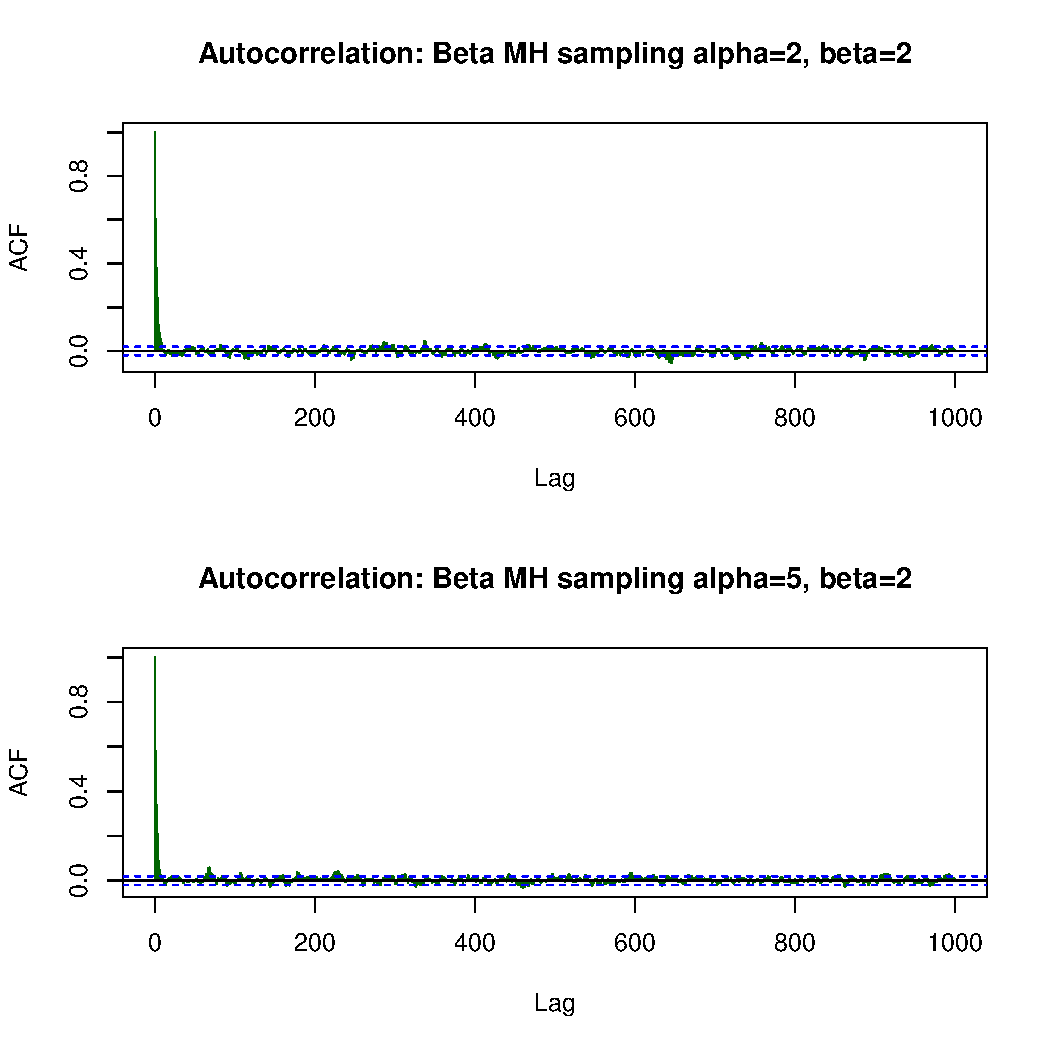
\includegraphics[width=\maxwidth]{figure/acf_q3-1} \caption[Autocorrelation functions for two parameter scenarios for sampling from the beta distribution]{Autocorrelation functions for two parameter scenarios for sampling from the beta distribution.}\label{fig:acf_q3}
\end{figure}


\end{knitrout}

\end{document}
